\section{Numerical Experiments}\label{sec:exp}
The experiments were carried out on \angus{insert details of machine and OS here}. All code was implemented and executed in MATLAB\angus{version number}, with kriging and co-kriging models constructed using the ooDACE toolbox~\cite{oodace}.

The \AlgName{} algorithm was compared against a baseline co-kriging algorithm. Both algorithms were run 30 times on each problem instance for the equivalent of 2000 low-fidelity evaluations, recording the best objective value, the mean and standard deviation of the resulting solutions produced by each run.


\subsection{Datasets}
The experiments were run on a collection of bound-constrained, single-objective, multi-fidelity test functions that can be divided into two different datasets. The first set (dataset $A$) is a selection of problem instances taken from Lv~et~al.~\cite{lv2021multi}. Problems $f10$ to $f17$ were chosen from this dataset as they contain between three and eight decision variables, determined as a representative range of easy to difficult problems. The problem instances here are provided with explicit definitions for both the high- and low-fidelity functions.

The second set of problem instances (dataset $B$) is generated using the Griewank~\cite{griewank1981generalized} and Michalewicz~\cite{michalewicz2013genetic} test problems (Figures~\ref{fig:grie} and~\ref{fig:michal}), taken from the literature. Each problem was instantiated with versions for three, five and eight decision variables. This matches the range of the first dataset, and also allows the performance of the algorithms to be judged across different sized problems in a more controlled environment. These test problems are not naturally multi-fidelity optimisation problems, so low-fidelity evaluations must be made by applying the methods described in~\cite{wang2017generic}. Two different error functions were tested for each instance, modelling two types of fidelity error: resolution and stochastic. An appropriate fidelity level $\phi$ for each problem was chosen by computing the square of the Pearson correlation coefficient $r^2$ for different fidelity values and selecting a value for $\phi$ such that $r^2$ was between 0.65 and 0.85, to be commensurate with the first dataset.

See Tables~\ref{tab:funcs} and~\ref{tab:errfuncs} in Appendix~\ref{app:testfuncs} for test function and error function equations, respectively.

\begin{figure}[h!]
  \centering
  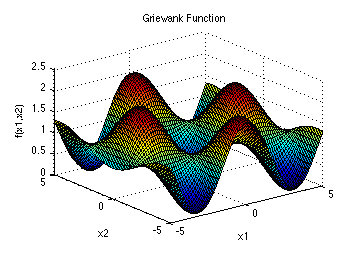
\includegraphics[width = 0.40\textwidth]{img/griewank.png} 
  \caption{The Griewank test function in 2D.\angus{will do a better version}} 
    \label{fig:grie}
\end{figure}
\begin{figure}[h!]
  \centering
  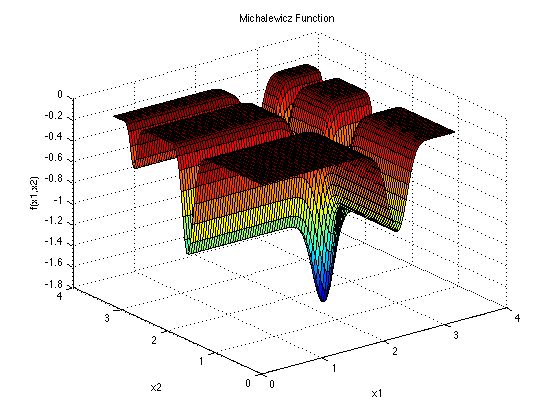
\includegraphics[width = 0.40\textwidth]{img/michal.png} 
  \caption{The Michalewicz test function in 2D.\angus{will do a better version}} 
    \label{fig:michal}
\end{figure}

\subsection{Baseline co-kriging algorithm}
Co-kriging is a popular approach to solving many multi-fidelity problems. The outer-loop of the \AlgName{} algorithm functions by iteratively updating a co-kriging model using data from a modified version of the OCBA procedure. In order to demonstrate the effectiveness of this new technique, the performance of \AlgName{} is compared against the baseline simple co-kriging algorithm given in Algorithm~\ref{alg:co-kriging}.

\begin{algorithm}[h!] 
\caption{Baseline co-kriging procedure}
\label{alg:co-kriging}
\algsetup{linenosize=\footnotesize}
{\footnotesize
\begin{algorithmic}[1]
\REQUIRE{$P$, problem data; $N_{L_{max}}$, max size of LF pop; $N_{e_{max}}$, maximum number of evaluations; $\Delta$, new LF per iteration.}
\ENSURE{Best solution found $\V{x}^\beta$.}
\STATE{$X_v \ot LHS(P),\ \forall v \in \{L,H\}$} \COMMENT{Generate initial populations}
\STATE{$\V{x}^\beta \ot \emptyset$} \COMMENT{Initialize $x_\beta$} 
\WHILE{$N_e < N_{e_{max}}$}
  \STATE{$A_L \ot A_L \cup LHS(\Delta)$} \COMMENT{Add $\Delta$ new solutions to LF archive}
  \IF{$|A_L| > N_{L_{max}}$}
    \STATE{$A_L \ot winnow(A_L,N_{L_{max}})$} \COMMENT{Control population size}
  \ENDIF
  \STATE{$M_C \ot CoKrige(A_L,A_H)$} \COMMENT{Update co-kriging model}
  \STATE{$\V{x} \ot GlobalSearch(M_C)$} \COMMENT{Globally search co-kriging model}
  \STATE{$\V{\alpha},N_e \ot f_H(\V{x},N_e)$} \COMMENT{Evaluate and update total cost}
  \STATE{$A_H \ot A_H \cup \{\V{\alpha}\}$} \COMMENT{Add $\V{\alpha}$ to high-fidelity archive}
  \STATE{$\V{x}^\beta \ot \min(f_H(\V{x}^\beta),f_H(\V{x}))$} \COMMENT{Update best solution}
\ENDWHILE
\end{algorithmic}
}
\end{algorithm}

The functions here have the same definitions as in Algorithm~\ref{alg:main-alg}. This procedure iteratively updates a co-kriging model by randomly sampling the low-fidelity data using a latin hypercube sampling (LHS) technique; however, the global search method remains the same.

\subsection{Parameters}
\AlgName{} can be viewed as a general framework into which various search and modeling methods can be ``plugged''. Therefore, its components can be divided into two categories: \AlgName{} specific components, which are intrinsic to its operation and whose parameters are also intrinsic; and, generic method components, such as global search techniques and modelling methods which can be substituted for other similar techniques, which come with their own parameters. The \AlgName{} specific parameters are discussed in Section~\ref{sec:method}; this section will detail the parameters for the generic search method used.

Differential evolution (DE) was used to globally search the updated co-kriging model. This DE was run over 30 generations with a crossover rate of 0.9, a mutation factor of 0.5 and a population size of 100.

The kriging models used are from the ooDACE toolbox~\cite{oodace}, with the default paramters.